%R.S.
\documentclass[format=acmsmall, review=false]{acmart}

\usepackage{acm-ec-17}
\usepackage{booktabs} % For formal tables

\usepackage{amsmath,amsfonts,amsmath,amsthm}
\usepackage{graphicx}
\usepackage{comment}
%\usepackage{wasysym}
%\usepackage{hyperref}
\usepackage{xcolor}
\usepackage[noend]{algpseudocode}
\usepackage{algorithm}
\usepackage{bm,esvect}

\newcommand{\inp}{I}
\newcommand{\out}{O}

\newcommand{\vtext}[1]{\begin{sideways}\parbox{23mm}{#1}\end{sideways}}
\newcommand{\ppre}{\textnormal{\textsf{pre}}}
\newcommand{\pre}{\textnormal{\textsf{CPre}}}
\newcommand{\cpre}{\textnormal{\textsf{CPre}}}
\newcommand{\preMP}{\widehat{\textnormal{\textsf{CPre}}}}
\newcommand{\prein}{\textnormal{\textsf{Pre}}_\inp}
\newcommand{\crit}{\textnormal{\textsf{Crit}}}
\newcommand{\critcpre}{\textnormal{\textsf{CritCPre}}}
\newcommand{\preout}{\textnormal{\textsf{Pre}}_\out}

\newcommand{\epre}{\textnormal{\textsf{EPre}}}
\newcommand{\apre}{\textnormal{\textsf{APre}}}
\newcommand{\xpre}{\textnormal{\textsf{XPre}}}

\newcommand{\reach}{\textnormal{\textsf{Reach}}}

\newcommand{\maxel}[1]{\lceil #1 \rceil}
\newcommand{\minel}[1]{\lfloor #1 \rfloor}
\newcommand{\useful}{\textnormal{\text{useful}}}

\newcommand{\lab}{\textnormal{\text{lab}}}
\newcommand{\outcome}{\textnormal{\textsf{outcome}}}
\newcommand{\Outcome}{\textnormal{\textsf{Outcome}}}

\newcommand{\finp}{\mathcal{F}_\inp}
\newcommand{\fout}{\mathcal{F}_\out}

\newcommand{\fc}{\mathcal{F}_1}
\newcommand{\fe}{\mathcal{F}_2}

\newcommand{\fm}{\mathcal{F}_m}

\newcommand{\conj}{\mathcal{C}}

\newcommand{\nat}{\mathbb{N}}

\newcommand{\strat}[1]{\langle\!\langle #1\rangle\!\rangle} 

\newcommand{\safe}{\textnormal{\textsf{Safe}}}
\newcommand{\win}{\textnormal{\textsf{Win}}}
\newcommand{\winpos}{\textnormal{\textsf{WinPos}}}
\newcommand{\plays}{\textnormal{\textsf{Plays}}}
\newcommand{\prefplays}{\textnormal{\textsf{PrefPlays}}}
\newcommand{\pref}{\textnormal{\textsf{Pref}}}
\newcommand{\ini}{\textnormal{\textsf{ini}}}
\newcommand{\last}{\textnormal{\textsf{last}}}
\newcommand{\first}{\textnormal{\textsf{first}}}
\newcommand{\Moves}{\textnormal{\textsf{Moves}}}
\newcommand{\MP}{\textnormal{\textsf{MP}}}
\newcommand{\mynote}[1]{\marginpar{$\spadesuit$ #1 $\spadesuit$}}


\newcommand{\clos}{\downarrow\!\!}

\newcommand{\size}[1]{|#1|}

%% \newcommand{\EF}[1]{{\color{red} #1}}
\newcommand{\EF}[1]{#1}

\newcommand{\good}{\textnormal{\textsf{good}}}
\newcommand{\Good}{\textnormal{\textsf{Good}}}
\newcommand{\choice}{\textnormal{\textsf{c}}}
\newcommand{\rep}{\textnormal{\textsf{rep}}}

\newcommand{\prop}{\textnormal{\textsf{P}}}

\newcommand{\suc}{\textnormal{\textsf{succ}}}
\newcommand{\pred}{\textnormal{\textsf{Pre}}}
\newcommand{\LTL}{\textnormal{\textsf{LTL}}\xspace}
%% \newcommand{\max}{\textnormal{\text{max}}}

\newcommand{\bound}{\ensuremath{2n(n^{2n+2}+1)}}

\newcommand{\until}{\,\mathcal{U}}
\newcommand{\always}{\Box}
\newcommand{\eventually}{\Diamond}

\newcommand{\true}{\ensuremath{\textsf{true}}\xspace}
\newcommand{\false}{\ensuremath{\textsf{false}}\xspace}

\newcommand{\uca}{\text{uc}}
\newcommand{\nba}{\text{b}}

\newcommand{\eop}{\ensuremath{\hfill\square}}

\newcommand{\NBW}{{\sf NBW}\xspace}
\newcommand{\UCW}{{\sf UCW}\xspace}
\newcommand{\UCT}{{\sf UCT}\xspace}
\newcommand{\AWT}{{\sf AWT}\xspace}
\newcommand{\NBT}{{\sf NBT}\xspace}
\newcommand{\UCWK}{{\sf U\textit{K}CW}\xspace}
\newcommand{\tb}{{\sf tb}}

\newcommand{\final}{\alpha}

\newcommand{\runs}{\textsf{Runs}}
\newcommand{\visit}{\textsf{Visit}}

\newcommand{\ourtool}{{\sf Acacia}\xspace}
\newcommand{\Lily}{{\sf Lily}\xspace}
\newcommand{\anzu}{{\sf Anzu}\xspace}
\newcommand{\rulebase}{{\sf RuleBase}\xspace}

\newcommand{\Obs}{{\sf Obs}}

\newcommand{\tuple}[1]{\langle #1 \rangle}

\newcommand\inter[1]{\llbracket #1 \rrbracket}

% from Laurent
\newcommand{\abs}[1]{\ensuremath{\lvert #1\rvert}}
\newcommand{\obs}{{\sf obs}}
\newcommand{\init}{{\sf init}}
\newcommand{\Allow}{{\sf Allow}}
\newcommand{\post}{{\sf post}}
\def\mynote#1{{\sf $\clubsuit$ #1 $\clubsuit$}}


%\newtheorem{theorem}{Theorem}
%\newtheorem{lemma}{Lemma}
%\newtheorem{remark}{Remark}
%\newtheorem{corollary}{Corollary}
%\newtheorem{proposition}{Proposition}
%\theoremstyle{definition}
\newtheorem{claim}[theorem]{Claim}

\newcommand{\abheek}[1]{{\color{red} U: #1}}


\begin{document}
% Title portion. Note the short title for running heads 
\title[DTEC]{DTEC: A new equilibria checker for omega-regular games}
\author{Abheek Ghosh}
\affiliation{%
  \department{Department of Computer Science}
  \institution{The University of Texas at Austin}
  %\streetaddress{104 Jamestown Rd}
  \city{Austin}
  \state{TX}
  %\postcode{400 005}
  \country{US}
}

%%% First abstract commented out


\begin{abstract}
We create an equilibria checker for finite multiplayer $\omega$-regular games called Doomsday-Threatening Equilibria Checker (DTEC). In a doomsday equilibrium, players use a strategy profile where all players satisfy their own objective, and if any coalition of players deviates and violate a player's objective then the objective of every player is violated. \cite{chatterjee2014doomsday} introduced this equilibria concept and gave algorithms and complexity results for deciding its existence for various classes of $\omega$-regular objectives.

DTEC has been implemented from scratch in C++. It provides a flexible and robust language to specify multiplayer graph games, comparable to popular model checking tools like NuSMV, Prism, Slugs, etc. It takes two input files, one that specifies the model, and the other gives the specifications. DTEC supports only reachability objectives, mainly because other, general, objectives have a bad time complexity as proved by \cite{chatterjee2014doomsday}. We also provide several examples that will help users create their own models and test them using the tool.

We also study several models for a four way traffic intersection. We observe that many reasonable models don't have a doomsday equilibrium, and finally refine them to get one that does have the equilibria. This project and the relevant papers we read introduced us to the area of finite multiplayer $\omega$-regular games.
\end{abstract}

\maketitle

\section{Introduction}
Two-player games have been very popular and useful for reactive synthesis~\cite{shapley1953stochastic,emerson1991tree,martin1975borel}. In these games, it is usually assumed that one of the players, the system, plays with the objective to satisfy some given specifications. While the other player, which consists of all the other players or components in the environment, is assumed to be adversarial and wants to violate the specifications. But it has been observed that in many scenarios, like protocol synthesis, it is more realistic to assume that the players may have their own objectives, and may or may not be adversarial to each other. This has increased the recent interest in multiplayer games~\cite{dana2010book,ummels2011complexity,chatterjee2006secure}.

Nash equilibrium is the concept popularly used to capture rational behavior in multiplayer settings --- the players are want to satisfy their own objective and are indifferent to other's objective~\cite{Nash48}. In areas outside verification and synthesis, like economics and algorithmic game theory, it is fine to assume that the players are indifferent to the objectives of other player or even altruistic (Stackelberg games), and therefore Nash equilibrium and its modifications like Bayes-Nash equilibrium, correlated equilibrium, etc. are popularly used. But in synthesis, it may be more appropriate to assume adversarial external criteria, captured by concepts like secure equilibria, doomsday-threatening equilibria, etc.~\cite{ummels2011complexity,chatterjee2006secure}.

\section{Doomsday-threatening Equilibria.}
There are $n$ players. The game is a tuple $(S, P, s_{{\sf init}}, \Sigma, \Delta, AP, L)$ such that 
\begin{itemize}
    \item $S$ is a nonempty finite set of \textit{states},
    \item $P=\{S_1,S_2,\dots,S_n\}$ is a partition of $S$ into $n$ classes of states, one for each Player~$i \in \{ 1,2,\dots,n\}$, 
    \item $s_{{\sf init}} \in S$ is the initial state, 
    \item $\Sigma$ is a finite set of alphabet,  
    \item $\Delta : S \times \Sigma \rightarrow S$ is the transition function of the game,
    \item $AP$ is the set of atomic propositions, and
    \item $L : S \rightarrow 2^{AP}$ is the function that labels each state.
\end{itemize}

The game starts from an initial state $s_{{\sf init}}$ and then it goes on infinitely. Each player $i$ has an LTL objective, say $W_i$. A player $i$ has control over states in $S_i$ and makes the move when the game is in those states. The strategy used by the player $i$ to make the moves, using the previous history, when the game is in $S_i$ is its strategy $\lambda_i$. Combining all the individual strategies, we get the strategy profile $\Lambda=(\lambda_1,\lambda_2,\dots,\lambda_n)$. When player $i$ plays using strategy $\lambda_i$, and others can play arbritarily, we get the set of paths $\outcome_i(\lambda_i)$. And given a strategy profile we get a fixed path $\outcome(\Lambda) = \bigcap \outcome_i(\lambda_i) $.

\paragraph{{\bf Doomsday-equilibrium}} A strategy profile $\Lambda=(\lambda_1,\lambda_2,\dots,\lambda_n)$ is a doomsday equilibrium (DE) if:
\begin{enumerate}
  \item All players satisfy their objective, i.e. for all $\outcome(\Lambda) \in \bigcap_i W_i$;

  \item and all players are able to retaliate in case of deviation: for all $i$, $1 \leq i \leq n$, for all path $\rho\in \outcome_i(\lambda_i)$, if
    $\rho\not\in W_i$, then $\rho \in \bigcap_{i\neq j} \overline{W_j}$. 

\end{enumerate}

The paper studies different types of LTL specification. For each of the types, it gives algorithms with different time complexities.
\begin{enumerate}
  \item Reachability objectives. Some set of states are visited eventually. Ptime-complete.
  \item Safety objectives. Some set of states are never left. Pspace-complete, NP-hard. Ptime for a fixed number of players.
  \item Buchi objectives. Always eventually some set of states is visited. Ptime-complete.
  \item Co-Buchi objectives. Eventually always some set of states is visited. Ptime-complete.
  \item Parity objectives. Let $d \in \nat$, a parity objective with $d$ priorities is a condition which is defined with a parity function $ p: S \rightarrow  \{0,1,\dots,d\}$ such that the minimal priority among the set of states that are visited infinitely often is even. Pspace, NP-hard, CoNP-hard.
\end{enumerate}

For different types of objectives, different algorithms are given. For tail objectives --- Buchi, co-Buchi, and parity --- there is an algorithm which works with different time complexity for the different cases. There is a second different algorithm for reachability objective, and another for safety objectives. For general LTL specification, the original problem is converted to a new larger problem, and the algorithm given for the parity objectives is used.

\section{DTEC}

As mentioned before, DTEC has been implemented from scratch in C++. DTEC can be divided into two main components:
\begin{itemize}
  \item The first part reads the .model and .specs files and constructs the model. DTEC supports a flexible and robust model specification format, similar to other tools like NuSMV, Prism, etc. This part of DTEC processes this model specification and sets up everything for the checker.
  \item The second part implements the algorithm~\ref{algo_reach} for reachability objective and checks whether a DE exists or not~\cite{chatterjee2014doomsday}. If an equilibrium exists, it also outputs a path that makes everyone reach their objective.
\end{itemize}

\begin{algorithm}
\caption{Equilibrium checking algorithm for reachability objectives.}\label{algo_reach}
\begin{algorithmic}[1]
\Require{Model, Reachability set for each player $T_i$}
\State{for all player $i$ do}
\State{\quad Find the set of states $F_i$, from which player $i$ has a strategy to force the game to eventually reach $T_i$ against all other players. (2-player reachability game)}
\State{\quad Find the set of states $R_i$, from which player $i$ has a strategy to always force doomsday ($\cap_j \overline{T_j}$) or $F_i$. (2-player safety game)}
\State{end for}
\State{Find a path that starts from $s_{{\sf init}}$ and stays in $\cap_i R_i$ until it reaches a state $s \in S$ such that $s \in T_i$ for some $i$ and $s \in \cap_j F_j$.}
\State \textbf{return} If such a path exists, return \textit{true}, else return \textit{false}.
\end{algorithmic}
\end{algorithm}

The model file has seven sections corresponding to the game tuple $(S, P, s_{{\sf init}}, \Sigma, \Delta, AP, L) \leftrightarrow $ (STATES, PARTITIONS, INITIAL STATE, ALPHABET, TRANSITION FUNCTION, ATOMIC PROPOSITIONS, LABELING FUNCTION). It has features like arrays, including negative range based indices, good lexicographic analysis, parsing, and error checking. The code has been submitted to Canvas, and it is also available at Github: https://github.com/AbheekG/dtec with usage instructions. The example $hello\_world$ ($hello\_world.model$ and $hello\_world.specs$) explains the usage along with a running example.

\section{Examples}
In this section, we provide some examples, most of them based on the traffic intersection.

\begin{example}\label{ex1}\cite{chatterjee2014doomsday}
Fair-Exchange Protocol 1 (first example given in the paper) [Files: $paper\_1.model$, $paper\_1.specs$]. There are two players: $A$ and $B$. They are exchanging items, like money or property. First, $A$ decides whether to give or not give (say property), then $B$ decides to give or not give (say money). They both want to receive the item (reachability specification for such a state) and would prefer not giving the item if possible.
\end{example}

\begin{example}\label{ex2}\cite{chatterjee2014doomsday}
Fair-Exchange Protocol 2 (second example given in the paper) [Files: $paper\_1.model$,$paper\_1.specs$]. This example is similar to \ref{ex1}, except that in this there is a third step where $A$ can cancel the deal and all transactions.

There are two players: $A$ and $B$. They are exchanging items, like money or property. First, $A$ decides whether to give or not give (say property), then $B$ decides to give or not give (say money), then $A$ executes a veto to go forward or cancel the deal. They both want to receive the item (reachability specification for such a state) and would prefer not giving their item if possible.
\end{example}

\begin{figure}
\caption{ Fair-Exchange Protocols 1 (\ref{ex1}) and 2 (\ref{ex2}) }
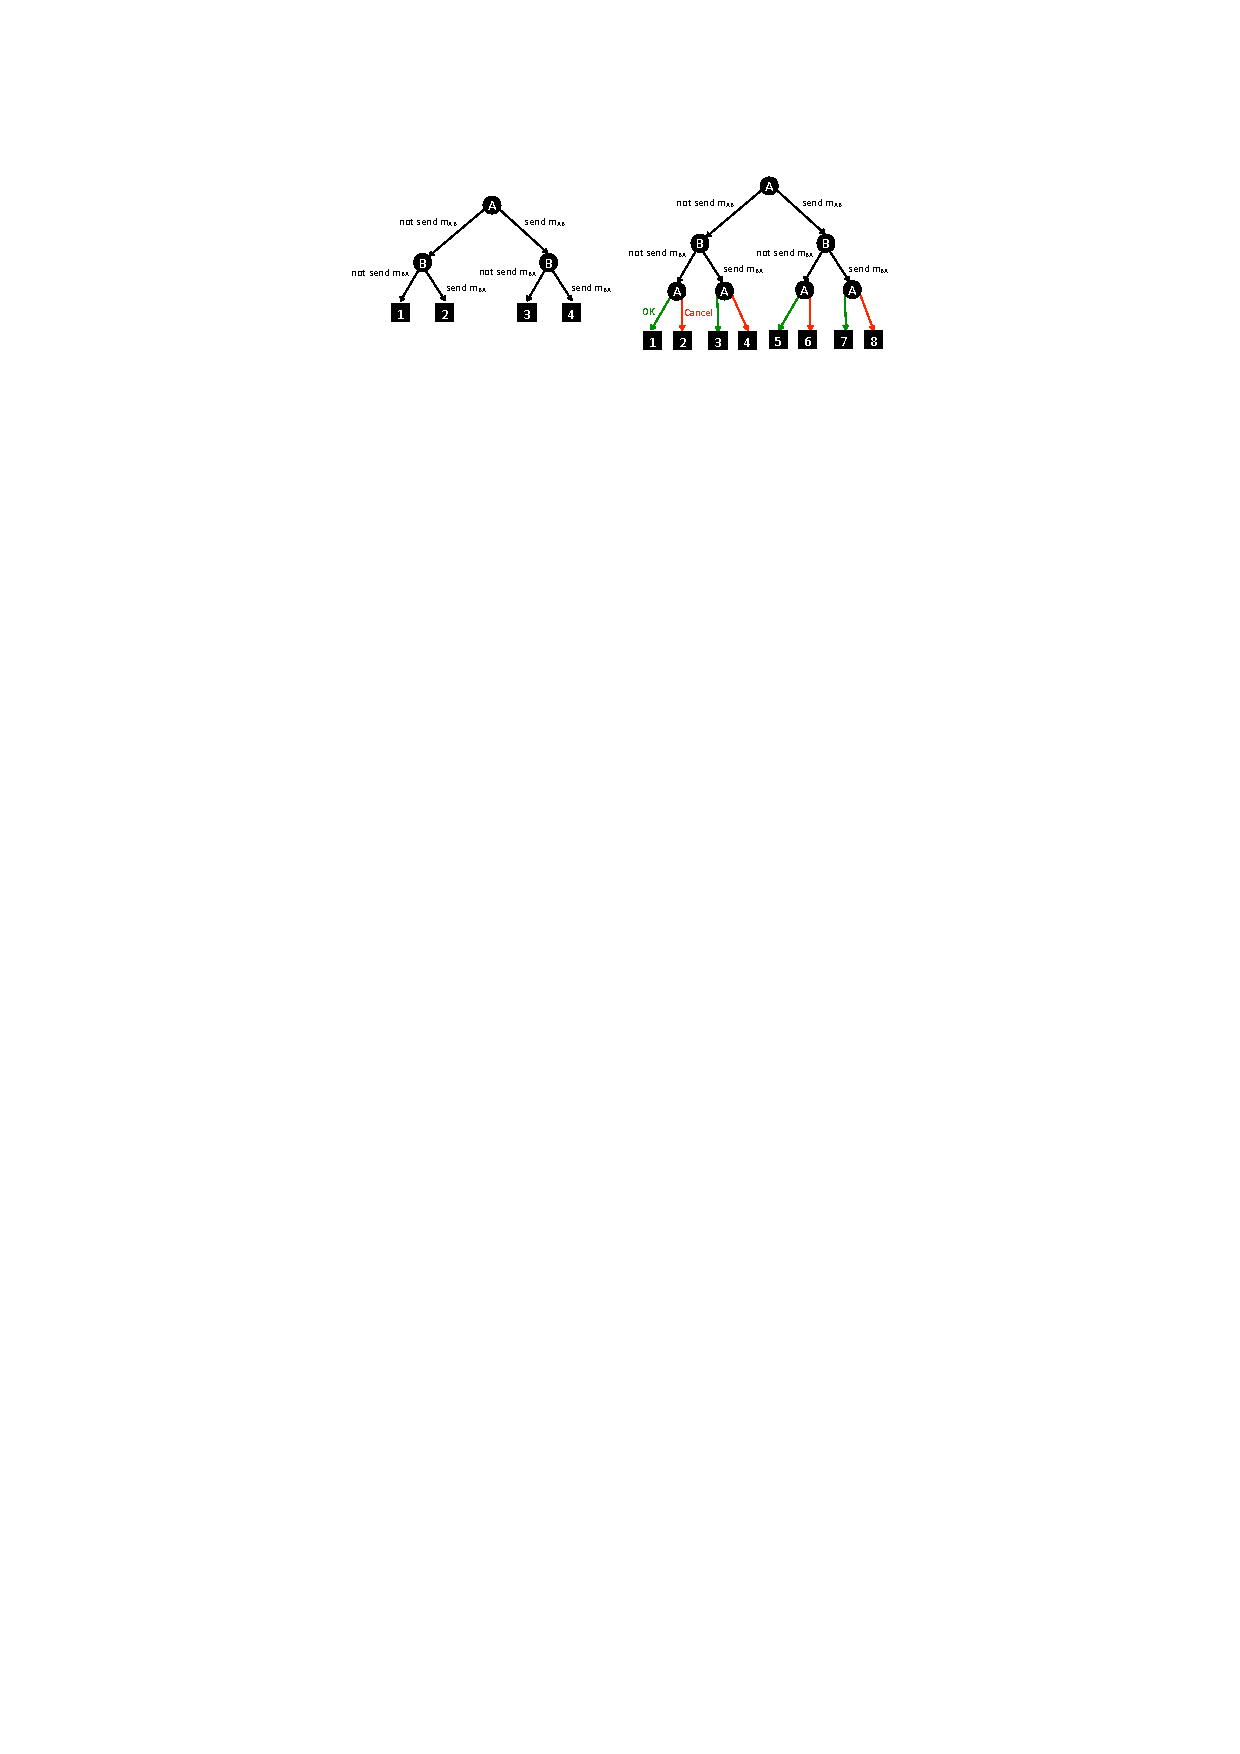
\includegraphics{fep}
\end{figure}

In Example \ref{ex1}, there doesn't exist any DE. Whether $A$ gives the property or not, $B$ has a dominating strategy to not give the money, which leaves $A$ with no option other than to not give the property. But in Example \ref{ex2}, there exists a DE. In the first step, $A$ decides to give the property, risk-free because it has the option to cancel the transaction later, and if it doesn't give the property then $B$ will also not give the money. If $A$ gives the property, then $B$ will give the money because otherwise, it knows that $A$ will cancel the transaction. And in the last step, $A$ doesn't cancel the transaction because doing that will cancel the transfer of both money and property.

\begin{example}\label{tex1}
Traffic Protocol 1 (No DE) [Files: $traffic\_1.py$ (generates the .model file), $traffic\_1.model$, $traffic.specs$]. Four-way intersection. Four types of cars. Only one can go at a time, if more than one goes at the same time then they collide.

Decide order: 1 - 2 - 3 - 4 - EXEC. This keeps on repeating infinitely.

Each car can decide to:
\begin{itemize}
\item W: Wait
\item G: Go
\end{itemize}

Each car can be in one of these four states:
\begin{itemize}
\item W: Waiting
\item G: Go
\item R: Reached
\item C: Crashed
\end{itemize}

Initially, everyone is in W (Waiting) state. While in W, if only one car decides G (Go), it reaches R (Reached). If more than one cars decide G (Go), the cars that decided to G (Go) reaches C (Crashed). Once a car is in R or C, it stays there. We assume that if some cars crash in the current time step (iteration), it doesn't affect the next time step and other cars can possibly reach successfully then.

The combined state is a tuple of five components. The first four components correspond to individual states of the four cars. And the last component specifies who makes the current move (who controls the state) and it ranges from 0 to 4. 1-4: the four players. 0: for the execution by the system depending upon previous moves (deterministic, no uncertainty). In our game there is no system, but we can assign the states belonging to the system to any arbitrary player as it doesn't create any problem because, as mentioned, the next state is fixed for any action.
\end{example}

The Traffic Protocol 1 (Example \ref{tex1}) doesn't have any DE. We present modified protocols in Examples \ref{tex2} to \ref{tex8}. Examples \ref{tex1} to \ref{tex6} don't have a DE, but Examples \ref{tex7} to \ref{tex8} have a DE.

\begin{example}\label{tex2}
Traffic Protocol 2 (No DE) [Files: $traffic\_2.py$ (generates the .model file), $traffic\_2.model$, $traffic.specs$]. The model is similar to Example \ref{tex1}, except now we give the cars multiple chances before each execution, and therefore more memory. We tried this to allow cars to collaborate, but doesn't help.

Order: 1 - 2 - 3 - 4 - 1 - 2 - 3 - 4 - ... - 4 - EXEC - (repeat)
\end{example}

\begin{example}\label{tex3}
Traffic Protocol 3 (No DE) [Files: $traffic\_3.py$ (generates the .model file), $traffic\_3.model$, $traffic.specs$]. Modification to \ref{tex2}, here when more than one cars G (Go), then they don't C (Crash) but again reset to W (Waiting).
\end{example}

\begin{example}\label{tex4}
Traffic Protocol 4 (No DE) [Files: $traffic\_4.py$ (generates the .model file), $traffic\_4.model$, $traffic.specs$]. Modification to \ref{tex2}. As explained in \ref{tex2}, the cars have multiple time points to decide their move before each execution and they could only take action from W (to W or G), now they are allowed to go from G to W also.
\end{example}

\begin{example}\label{tex5}
Traffic Protocol 5 (No DE) [Files: $traffic\_5.py$ (generates the .model file), $traffic\_5.model$, $traffic.specs$]. As we are finding it difficult to get a model with a DE, we go back to Traffic Protocol 1 (\ref{tex1}) and further make it easier to find a DE. We allow car 1 and car 3 to pass simultaneously without crashing, same for car 2 and car 4. It follows from the real-life observation that the opposite ways (like North-South, East-West) can go straight simultaneously.
\end{example}

\begin{example}\label{tex6}
Traffic Protocol 6 (No DE) [Files: $traffic\_6.py$ (generates the .model file), $traffic\_6.model$, $traffic.specs$]. The model is similar to Traffic Protocol 2 (Example \ref{tex2}), where we gave the cars multiple chances before each execution, but now we also add a booking round after each iteration. So the order of steps looks like:

1 - 2 - 3 - 4 - BOOK - 1 - 2 - 3 - 4 - BOOK - ... - 4 - BOOK - EXEC - (repeat)

There is also a state B (Booked) for the cars, in addition to the previous four: W, G, R, and C. If there is only one G (Go) in a given iteration, then the booking step (BOOK) makes the car's state B (Booked), otherwise if multiple cars select G then they all reach C (Crashed). In the final execution step (EXEC), all the B (Booked) cars reach R (Reached).
\end{example}

\begin{example}\label{tex7}
Traffic Protocol 7 (DE exists!) [Files: $traffic\_7.py$ (generates the .model file), $traffic\_7.model$, $traffic.specs$]. The model has all the components of Traffic Protocol 6 (Example \ref{tex6}), like multiple steps before execution (EXEC) and booking (BOOK), additionally, this new model has a Veto iteration before the EXEC. Now the order of steps look like:

1 - 2 - 3 - 4 - BOOK - 1 - 2 - 3 - 4 - BOOK - ... - 4 - BOOK - Veto1 - Veto2 - Veto3 - Veto4 - EXEC - (repeat)

In the Veto iteration, a car can cancel all bookings, i.e., all B (Booked) cars go back to W (Waiting). This allows a car to create doomsday if it doesn't get booked. If the number of booking iterations is greater than or equal to the number of cars, then they reach a DE.
\end{example}

\begin{example}\label{tex8}
Traffic Protocol 8 and 9 (DE exists!) [Files: $traffic\_8.py$ and $traffic\_9.py$ (generates the .model file), (the model is not attached due to large size (\~1 GB) but can be generated using the .py file), $traffic_8.specs$ and $traffic_12.specs$]. This is similar to Traffic Protocol 7 (Example \ref{tex7}) with the additional feature of selective crashing as introduced in Example \ref{tex5} and twelve types of cars going:
\[\{East,West,North,South\} x \{Left,Right,Straight\}\]. In 

For example, cars going East-Straight and West-Straight don't crash, but cars going East-Stright and West-Left crash. In these examples, if the number of booking iterations is greater than or equal to four (less than types of cars), then they reach a DE.
\end{example}

\section{Conclusion}

In the examples, we saw the types of models that can have a DE and also the ones that don't. In the first six traffic examples, it can be observed that for the car 1, there was no move that could guarantee R (Reached) for itself or C (Crashed) for all. If the car 1 decided G (Go) then it could be crashed by some other car and they both could reach C, while some other car can reach R in some other iteration. But in the last few examples, by giving the veto power to the cars/players and having a sufficient number of booking rounds, all cars can book a slot and successfully reach their destination.

The DTEC has an easy and robust input language and can be used for checking DE with reachability objectives by researchers in the area. We also learned about multiplayer games and their relation with formal methods and reactive synthesis.

\bibliographystyle{ACM-Reference-Format}

\bibliography{references}

\end{document}


